\rhead{\bf MC\_Initialize()}
\label{api:MC_Initialize}
\noindent
\vspace{5pt}
\rule{6.5in}{0.015in}
\noindent
{\LARGE \bf MC\_Initialize()\index{MC\_Initialize()}}\\
\phantomsection
\addcontentsline{toc}{section}{MC\_Initialize()}

\noindent
{\bf Synopsis}\\
{\bf \#include $<$libmc.h$>$}\\
{\bf MCAgency\_t MC\_Initialize}({\bf int} $port$, {\bf MCAgencyOptions\_t} $*options$);\\

\noindent
{\bf Purpose}\\
Start a Mobile-C agency and return a handle of the launched agency.\\

\noindent
{\bf Return Value}\\
The function returns an {\bf MCAgency\_t} on success and NULL on failure.\\

\noindent
{\bf Parameters}
\vspace{-0.1in}
\begin{description}
\item
\begin{tabular}{p{10 mm}p{145 mm}}
$port$ & The port number to listen on for incoming mobile agents.\\
$options$ & The address of a structure of type {\bf MCAgencyOptions\_t} for 
specifying which thread(s) to be activated in an agency and setting the 
default agent status for incoming mobile agents.
\end{tabular}
\end{description}
{\bf MCAgencyOptions\_t} is defined as a structure as the following:
\verbatiminput{api/MCAgencyOptions_t.txt}

\noindent
{\bf Description}\\
\texttt{MC\_Initialize()} starts a Mobile-C agency and returns a handle of 
type \texttt{MCAgency\_t} containing the information about the current agency.

The \texttt{MC\_Initialize} function also accepts an optional argument of type
\texttt{MCAgencyOptions\_t} which allows a user to modify which components to
start on their Mobile-C agency. The \texttt{MCAgencyOptions\_t} struct should be initialized with the 
\texttt{MC\_InitializeAgencyOptions} before modifications are made. The struct contains the following
members:
\begin{itemize}
  \item \texttt{int threads;} : This member is a bitmasked variable which contains information
  about which Mobile-C threads to start upon startup. The bits are organized as such:

  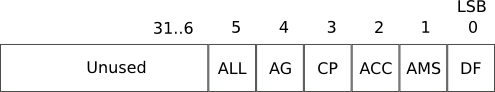
\includegraphics[width=4in]{figure/mobilec_threads_bitfields.png} 
  
  with the following acronyms:
    \begin{itemize}
      \item LSB: Least SignificantBit
      \item DF: Directory Facilitator
      \item AMS: Agent Management System
      \item ACC: Agent Communication Channel
      \item CP: Command Prompt
      \item AG: Agent Threads
    \end{itemize}
    A value of ``1'' in a bitfield tells Mobile-C to enable a particular thread,
    and a value of ``0'' informs Mobile-C not to activate that thread upon
    startup. A set of enumerations are defined in libmc.h that define the macros 
    \texttt{MC\_THREAD\_DF, MC\_THREAD\_AMS}, \texttt{MC\_THREAD\_ACC, MC\_THREAD\_CP, MC\_THREAD\_AGENT},
    each representing the bit position of each thread. There is also a 
    special macro, \texttt{MC\_THREAD\_ALL}, which represents the total number of 
    types of threads in a Mobile-C agency. For instance, to disable
    the command prompt thread, the following code may be used:
    \begin{verbatim}
    options.threads &= ~(1 << MC_OPTIONS_CP);
    \end{verbatim}
    where \texttt{options} is a struct of type \texttt{MCAgencyOptions\_t}.

    Helper functions \texttt{MC\_SetThreadOn(), MC\_SetThreadsAllOn(),
    MC\_SetThreadOff(), MC\_SetThreadsAllOff()} are also provided to modify the
    threads to start. Please consult their repsective documentation pages for
    more information.

  \item \texttt{int default\_agent\_status;} : This is the default agent status
  to assign to all incoming agents. Valid agent status values are found in
  \texttt{libmc.h} under the enumeration \texttt{MC\_AgentStatus\_e}. Possible
  values are:
    \begin{itemize}
    \item \texttt{MC\_WAIT\_CH} : This denotes that the agent is waiting for the
    next available Ch interpereter so that it may execute. This is the default
    setting for all incoming agents.
    \item \texttt{MC\_WAIT\_MESSGSEND} : This agent status indicates that the
    agent has finished its local task, but still has more remote tasks remaining.
    An agent with this status is waiting to be handled by the ACC so that it may
    migrate to the location of its next task.
    \item \texttt{MC\_AGENT\_ACTIVE} : This indicates that the agent is currently
    executing.
    \item \texttt{MC\_AGENT\_NEUTRAL} : This indicates that the agent is not
    executing, but is also not waiting for service. The agent simply persists 
    in the agency. This option is also a popular default alternative to
    \texttt{MC\_WAIT\_CH} since incoming agents are not executed upon arrival.
    \item \texttt{MC\_AGENT\_FINISHED} : This agent status indicates that the
    agent has finished all of its tasks and is awaiting to be purged from the
    agency.
    \end{itemize}
  \item \texttt{int modified;} : This member field is unused.
  \item \texttt{int enable\_security;} : This indicates that the Mobile-C agency
  should enable the Mobile-C security processes. This member is off by default.
  \item \texttt{unsigned char passphrase[32]} : This is a character string a
  passphrase to decrypt the agency's private key. For more details about the
  Mobile-C security process, please refer to Chapter \ref{chap:Security}.
  \item \texttt{int stack\_size[MC\_THREAD\_ALL];} : (Unix only) This array of integers holds
  the stack size to allocate for each thread. For example, if the programmer
  knows in advance that all agents the agency will receive will be small, the
  programmer may limit the stack size of each agent thread to one kilobyte with
  the following line:
  \begin{verbatim}
  options.stack_size[MC_THREAD_AGENT] = 1024;
  \end{verbatim}
  Care should be taken when modifying stack sizes as it may cause instability
  in the system. 
  \item \texttt{char *known\_host\_filename;} : (Optional) This should point to
  a filename containing host names of known and trusted hosts. This file is only
  used if Mobile-C security is enabled.
  \item \texttt{char *priv\_key\_filename;} : (Optional) This should point to a
  string containing the filename of the agency's private key file. This is only
  used if Mobile-C security is enabled.
  \item \texttt{ChOptions\_t* ch\_options;} : This may be used to modify Ch 
  options for agency interpreters. Please refer to the Embedded Ch documentation
  for more information about \texttt{ChOptions\_t}.
\end{itemize}

\noindent
{\bf Example: Starting an agency with default options}\\
\noindent
{\footnotesize\verbatiminput{../demos/getting_started/hello_world/server.c}}

{\bf Example: Starting an agency with no command prompt}\\
\noindent
{\footnotesize\verbatiminput{../demos/FIPA_compliant_ACL_messages/fipa_test/client.c}}

\noindent
{\bf See Also}\\
MC\_End()

%\CPlot::\DataThreeD(), \CPlot::\DataFile(), \CPlot::\Plotting(), \plotxy().\\
